\subsection{مقدمه}

به طور کلی می‌توان جایگاه روش‌های مبتنی بر یادگیری عمیق را در حوزه تولید شرح متناظر تصویر، از سال 2014 به بعد به روشنی در میان پژوهش‌های انجام‌شده مرتبط با این موضوع دریافت. از حدود سال 2013 و 2014، روش‌های مبتنی بر یادگیری عمیق، عمل‌کرد بسیار مناسب‌تری نسبت به روش‌های مبتنی بر مدل‌های گرافی احتمالاتی در این زمینه از خود نشان داده‌اند که این امر موجب استقبال چشم‌گیر پژوهش‌گران از این ایده شد.
\\
 استفاده از شبکه‌های عصبی و یادگیری عمیق به طور عمده در هر دو مرحله درک صحنه و تولید جمله در بین پژوهش‌های زیادی به چشم می‌خورد. با این حال، در مرحله درک صحنه تقریبا تمام پژوهش‌های انجام شده با استفاده از یک شبکه عصبی کانولوشنی عمیق، اقدام به استخراج بردار ویژگی تصویر می‌نمایند و این بردار ویژگی را به مرحله تولید جمله ارسال می‌کنند. بر خلاف مرحله درک صحنه که ایده‌های مطرح‌شده در آن از تنوع کم‌تری برخوردار است، مرحله تولید جمله چالشی‌ترین بخش فرایند به‌شمار می‌رود. 
 \\
 در بخش‌های قبلی به طور جداگانه به بررسی روش‌های مبتنی بر یادگیری عمیق ارائه شده برای تک‌تک مراحل  پرداختیم. با این حال، روش‌های ارائه شده در این بخش‌ها عموما روش‌های پایه‌ای هستند که بهبودهای زیادی روی هر یک از آن‌ها انجام شده است. در این بخش به بیان روش‌های جدیدتر و پیچیده‌تر در این حوزه خواهیم پرداخت.
 \\
از جمله پژوهش‌هایی که با تکیه بر شبکه‌های عصبی و یادگیری عمیق اقدام به تولید شرح متناظر تصویر نموده است، می‌توان به پژوهش \cite{karpathy2015deep} اشاره کرد که توسط خانم لی و همکارانش در سال 2015، ارائه شده و با استفاده از شبکه‌های عصبی کانولوشنی عمیق و دو نوع از شبکه‌های عصبی بازگشتی موسوم به شبکه‌های عصبی بازگشتی مالتی‌مودال و شبکه‌های عصبی بازگشتی دوطرفه، روش مناسبی برای تولید خودکار شرح بر تصاویر ارائه داده است.
\\
در این پژوهش، ابتدا با بهره‌گیری از روش شبکه عصبی کانولوشنی ناحیه‌ای، نواحی از تصویر که شامل تصویر اجسام است، استخراج شده و با استفاده از یک شبکه عصبی کریشفسکی، بردار ویژگی برای هر ناحیه محاسبه می‌شود. سپس با بهره‌گیری از یک شبکه عصبی بازگشتی دوطرفه، عبارات مختلف از جمله استخراج و بردارهای ویژگی برای هر عبارت محاسبه می‌شود. سپس با استفاده از یک تابع هدف و مدل میدان تصادفی مارکف، هم‌ترازسازی بین نواحی و عبارات زبانی صورت گرفته و مدل آموزش داده می‌شود.
\\
 در ادامه با تخمین بهینه پارامترهای موجود و با استفاده از شبکه عصبی بازگشتی مالتی‌مودال، توزیع احتمال بهترین کلمه بعدی در یک جمله با داشتن کلمات قبلی و محتوای حاصل از بردار ویژگی محاسبه شده روی نواحی تصویر، محاسبه شده و بهترین کلمه بعدی تولید می‌شود. این کار تا جایی ادامه می‌یابد که شبکه، نشانه مخصوص پایان جمله را تولید کند.
  
 
 
 
 
 \subsection{تولید جمله با مفهوم مشخص}
استفاده از شبکه عصبی بازگشتی ضربی منجر به فراهم‌سازی بستری مناسب جهت تولید جمله در سطح حروف می‌شود. با این وجود برای تولید خودکار شرح بر تصاویر، نیازمند آن‌ هستیم که محتوای جملات را به طور مشخص و از پیش تعیین شده داشته باشیم. به همین دلیل نیاز به ارائه روش که طی آن بتوانیم معنا و محتوای جملات تولید شده توسط شبکه عصبی بازگشتی را کنترل کنیم، مشهود می‌شود.
\\
در پژوهش \cite{karpathy2015deep} روش جدیدی برا تولید شرح خودکار بر تصاویر ارائه شده است که در مرحله تولید جمله، از نوع خاصی از شبکه‌های عصبی بازگشتی موسوم به شبکه عصبی بازگشتی دوطرفه\enfootnote{Bidirectional RNN}، استفاده  شده است. در این روش، ابتدا از یک شبکه عصبی کانولوشنی عمیق بر روی نواحی استخراج شده از تصاویر برای استخراج ویژگی و درک صحنه استفاده شده است. از سوی دیگر، با اعمال یک شبکه عصبی بازگشتی دوطرفه بر جملات و ارائه یک تابع هدف ساختارمند، روشی برای هم‌ترازسازی جمله و اطلاعات بصری نهفته در تصویر ارائه شده است.
\\

شکل \ref{fig:deep1}، نمونه‌ای از هم‌ترازسازی ارائه شده در این پژوهش برای یک تصویر را نشان می‌دهد.
\begin{figure}[H]
\center
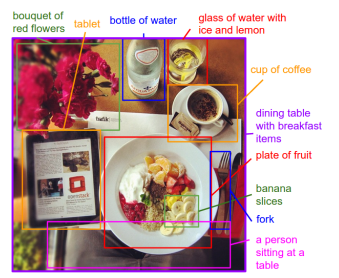
\includegraphics[scale=0.6]{Imgs/sentence_deep1.png}
\caption{هم‌ترازسازی تصویر و جمله\cite{karpathy2015deep}}
\label{fig:deep1}
\end{figure}

در مدل هم‌ترازسازی ارائه شده در این پژوهش، فرض بر این است که یک مجموعه‌داده شامل تعداد زیادی تصویر و جملات متناظر با هر تصویر وجود دارد. همین‌طور فرض دیگری وجود دارد مبنی بر این‌که بخش‌های مختلف هر جمله، به نواحی خاصی از تصویر اشاره‌ می‌کنند که موقعیت این نواحی مجهول است. از طرف دیگر اشاره این بخش‌ها به نواحی مرتبط خود در تصاویر، در بین تمام مجمو‌‌عه‌داده، تکرار می‌شود. به عنوان مثال، عبارات زبانی شامل کلمه «توپ» در تمام تصاویر موجود در مجموعه‌داده، به نواحی از تصویر اشاره می‌کنند که دارای ويژگی‌های «توپ» هستند.
\\
در شکل \ref{fig:deep2} ارتباط بین بخش‌های مختلف یک جمله و نواحی متفاوت از تصویر را مشاهده می‌نمایید. همان‌طور که در شکل مشاهده می‌شود، ابتدا برای تصاویر موجود در مجموعه‌داده و شرح متناظر با هر یک از این تصاویر، ارتباطات بین عبارات مختلف از جملات و نواحی تصاویر استخراج و یادگرفته می‌شود. در ادامه، با ورود یک  تصویر جدید و براساس ارتباطات یادگرفته شده، شرح جدید برای تصویر تولید می‌شود.

\begin{figure}[H]
\center
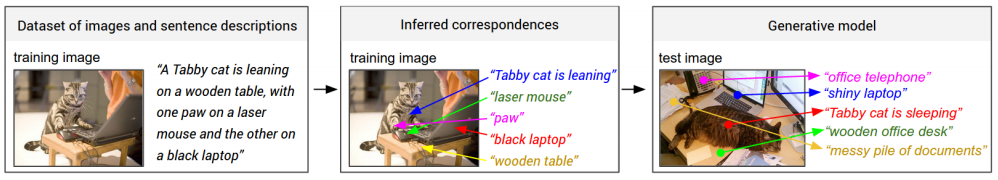
\includegraphics[scale=0.45]{Imgs/sentence_deep2.png}
\caption{ارتباط بین نواحی مختلف یک تصویر و عبارات جمله\cite{karpathy2015deep}}
\label{fig:deep2}
\end{figure}

برای تبدیل تصویر به فضای ویژگی، مطابق با آن‌چه در فصل درک صحنه ذکر شد، ابتدا با استفاده از روش شبکه‌های عصبی کانولوشنی ناحیه‌ای،‌ ۱۹ ناحیه از تصویر استخراج شده و برای ۲۰ تصویر موجود، با اعمال یک بهینه‌سازی و تخمین پارامتر و اعمال یک شبکه عصبی، بردار ویژگی استخراج می‌شود. پس از استخراج بردار ویژگی از نواحی تصویر، نیازمند آن هستیم که بتوانیم از عبارات مختلف جمله، بردار ویژگی هم‌اندازه با بردار ویژگی حاصل از تصویر، استخراج کنیم. برای این کار، در این پژوهش از شبکه‌ عصبی بازگشتی دوطرفه استفاده شده است. 
\\
این شبکه عصبی، یک دنباله از $N$ کلمه را به عنوان ورودی دریافت کرده و هر یک را به یک بردار در فضای $h$ بعدی، که $h$ اندازه بردار ویژگی حاصل از نواحی تصویر است، نگاشت می‌کند. رابطه \eqref{eq:deep1}، رابطه مربوط به پارامترهای این شبکه عصبی را نمایش می‌دهد.
در این رابطه، $I$ یک بردار ستونی اندیکاتور\enfootnote{Indicator} است که در اندیس کلمه $t$ام خود یک و در بقیه اندیس‌ها صفر دارد. $W_w$ یک ماتریس وزن ثابت برای هر کلمه $w$ است که برای جلوگیری از بیش‌برازش بر داده‌ها، مورد استفاده قرار می‌گیرد.

\begin{align*}
x_t &= W_{w} I_t 
\\
e_t &= f(W_ex_t + b_e)
\\
h_t^f &= f(e_t + W_fh_{t-1}^f + b_f)
\\
h_t^b &= f(e_t + W_bh_{t-1}^b + b_b)
\\
s_t &= f(W_d(h_t^f + h_t^b) + b_d)
\numberthis
\label{eq:deep1}
\end{align*}

 در این شبکه، دو جریان داده وجود دارد. جریان اول، جریان داده بین گر‌ه‌های مخفی شبکه از چپ به راست و دیگری جریان داده بین نود‌های مخفی شبکه از راست به چپ است که به ترتیب با $h_t^f$ و $h_t^b$ نمایش داده می‌شوند. بردار نهایی $s_t$، بردار حاصل از نگاشت کلمات به فضای ویژگی‌ها است که با استفاده از خود کلمه و محتوای مورد استفاده در اطراف کلمه در جمله، تولید می‌شود.
\\
شکل \ref{fig:deep3} طرح‌واره‌ای از معماری این شبکه را نمایش می‌دهد. همان‌طور که در این شکل مشخص است، در لایه مخفی این شبکه، دو جریان داده، یکی از راست به چپ و دیگری از چپ به راست برای محاسبه تاثیر کلمات اطراف کلمه جاری بر نگاشت کلمه به فضای ویژگی‌ها، وجود دارد.

\begin{figure}[H]
\center
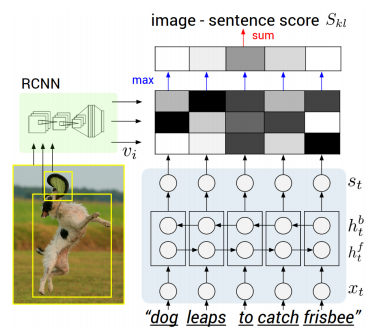
\includegraphics[scale=0.8]{Imgs/sentence_deep3.png}
\caption{طرح‌واره شبکه عصبی بازگشتی دوطرفه\cite{karpathy2015deep}}
\label{fig:deep3}
\end{figure}

 در ادامه با بهره‌گیری از روش نگاشت دوطرفه تصاویر و جملات که در بخش درک صحنه ارائه شد، توابع هم‌ترازسازی و تابع هدف ارائه شده را مورد استفاده قرار داده و با استفاده از روش یادگیری چند نمونه‌ای، اقدام به یادگیری انتساب‌های بین نواحی مختلف تصاویر و عبارات مختلف زبانی می‌شود.
 \\
 با استفاده از این روش، می‌توان برای هر ناحیه از تصویر، کلمات مناسب را تعیین کرد. اما برای تولید خودکار شرح بر تصاویر، نیاز به تولید عبارات زبانی وجود دارد. برای حل این مشکل، با در نظر گرفتن رابطه ضرب داخلی بین بردارهای ویژگی حاصل از نواحی تصویر و عبارات زبانی یک جمله به عنوان معیار شباهت، روشی ارائه شده است که بتوان برای هر ناحیه از تصویر، عبارت زبانی مناسبی تولید کرد.
 \\
 در این روش، با تعریف یک تابع انرژی و استفاده از مدل میدان تصادفی مارکف، با بهینه‌سازی تابع انرژی ارائه شده، بهترین هم‌ترازسازی برای هر یک از عبارات موجود محاسبه شده و عبارت با بهترین مقدار، انتخاب می‌شود. رابطه \eqref{eq:deep2}، این تابع انرژی را محاسبه می‌کند.
 
 
 \begin{align*}
 E(a) =  \ML{\Sigma}_{j=1\cdots N}\Psi_j^U(a_j) &+ \ML{\Sigma}_{j=1\cdots M}\Psi_j^B(a_j, a_{j+1})
 \\
 \Psi_j^U(a_j) &= \nu_i^T \cdot s^t
 \\
 \Psi_j^B(a_j,a_{j+1}) &= \beta I(a_j = a_{j+1})
 \numberthis
 \label{eq:deep2}
 \end{align*}


می‌توان در شکل \ref{fig:deep7} نتایج استفاده از این شبکه و محاسبه میزان شباهت نواحی مختلف تصویر و عبارات مختلف از جملات را مشاهده نمود. این شکل، نتیجه آموزش اختصاص نواحی مختلف تصویر به عبارات زبانی را نمایش می‌دهد.

\begin{figure}[H]
\center
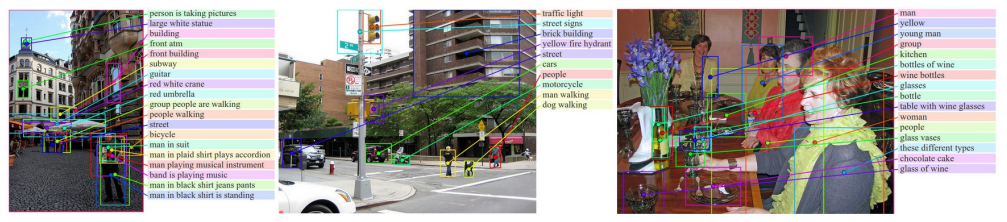
\includegraphics[scale=0.5]{Imgs/sentence_deep7}
\caption{انتساب نواحی مختلف تصویر به عبارات زبانی\cite{karpathy2015deep}}
\label{fig:deep7}
\end{figure}


تا این مرحله، با ورود یک تصویر، یا یک ناحیه از تصویر، عبارات زبانی متناظر، استخراج شده‌اند. هدف اصلی در این پژوهش تولید جمله برای هر تصویر است. بنابراین نیاز داریم تا با استفاده از مدل‌های ارائه شده برای تولید جمله، این کار را انجام دهیم. در پژوهش‌های زیادی، استفاده از شبکه‌های عصبی بازگشتی برای پیش‌بینی و محاسبه توزیع احتمال کلمه بعدی در یک جمله با در نظر داشتن کلمات قبلی و محتوای جمله، ارائه شده است. در این پژوهش با اعمال تغییرات کوچکی، از همین روش‌ها استفاده می‌شود. 
\\
رابطه ارائه شده برای شبکه عصبی بازگشتی که این کار را انجام می‌دهد، مطابق با رابطه \eqref{eq:deep3} است.
در این رابطه، $CNN_{\theta c}(IMAGE)$ بردار حاصل از اعمال آخرین لایه یک شبکه عصبی کانولوشنی بر تصویر را نشان می‌دهد و بقیه پارامترها، همگی قابل آموزش هستند. بردار $y_t$ بردار نماینده توزیع احتمالاتی تمام کلمات با در نظر گرفتن کلمات قبلی و محتوای هر ناحیه است که اندازه آن برابر است با تعداد تمام کلمات موجود در لغت‌نامه به علاوه یک نشانه خاص به عنوان «اتمام جمله».

\begin{align*}
b_\nu &= W_{hi}[CNN_{\theta c}(IMAGE)]
\\
h_t &= f(W_{hx}x_t + W_{hh}h_{t-1} + b_h + I(t = 1)\cdot b_\nu)
\\
y_t &= softmax(W_{oh}h_t + b_o)
\numberthis
\label{eq:deep3}
\end{align*}

شکل \ref{fig:deep4}، طرح‌واره‌ای از شبکه عصبی بازگشتی مالتی‌مودال\enfootnote{Multimodal} ارائه شده در این پژوهش برای تولید جمله را نمایش می‌دهد.

\begin{figure}[H]
\center
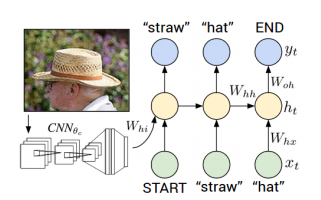
\includegraphics[scale=1]{Imgs/sentence_deep4.png}
\caption{طرح‌واره شبکه عصبی بازگشتی ارائه شده برا تولید جمله\cite{karpathy2015deep}}
\label{fig:deep4}
\end{figure}

جدول \ref{tbl:deep}
نتایج معیار \lr{BLUE} را برای روش ارائه شده بر روی سه مجموعه‌داده مختلف، نمایش می‌دهد. همان‌طور که در این جدول مشخص است، نتایج به دست آمده از این روش در مقایسه با دو روش دیگر، نتایج به نسبت بهتری بوده است.

\begin{table}[H]
\center
\caption{نتایج معیار \lr{BLUE} برای روش ارائه شده در \cite{karpathy2015deep} در مقایسه با دو روش دیگر}
\label{tbl:deep}
\begin{tabular}{c | c | c | c || c | c | c || c | c | c | c}
نام روش
&
\lr{B-1} &\lr{B-2} &\lr{B-3} &
\lr{B-1*} &\lr{B-2*} &\lr{B-3*} &
\lr{B-1**} &\lr{B-2**} &\lr{B-3**} &\lr{B-4**} 
\\
\hline
\hline
نزدیک‌ترین‌همسایه
&
ــ &ــ & ــ &
ــ &ــ & ــ &
45.0 &28.1 &16.6 &10.0
\\
روش \cite{mao2014explain}
&
58 & 28 & 23 &
55 & 24 & 20  &
ــ &ــ &ــ &ــ
\\
روش \cite{karpathy2015deep}
&
57.9 & 38.3 & 24.5 & 57.3 & 36.9 & 24.0 & 62.5 & 45.0 & 32.1 & 23.0 

\end{tabular}

\end{table}


شکل \ref{fig:deep5} نتایج رتبه‌بندی جملات و عبارات برای هر ناحیه از تصویر را نمایش می‌دهد.

\begin{figure}[H]
\center
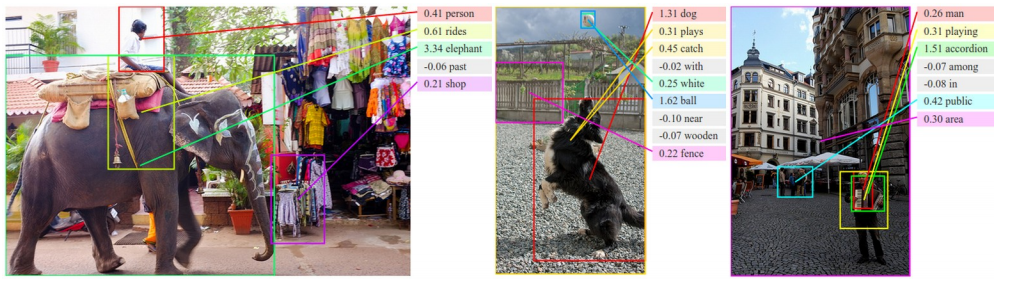
\includegraphics[scale=0.5]{Imgs/sentence_deep5.png}
\caption{نتایج رتبه‌بندی عبارات زبانی برای نواحی تصویر \cite{karpathy2015deep}}
\label{fig:deep5}
\end{figure}

به علاوه، در شکل \ref{fig:deep6} نتایج تولید شرح برای تصاویر، توسط شبکه عصبی بازگشتی ارائه شده در این پژوهش، به تصویر کشیده شده است.

\begin{figure}[H]
\center
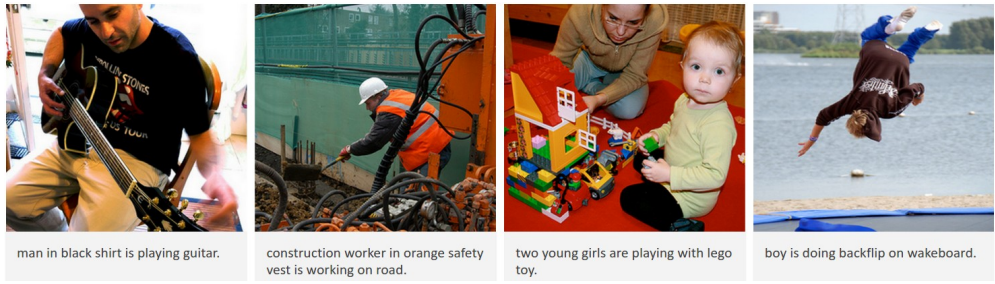
\includegraphics[scale=0.5]{Imgs/sentence_deep6}
\caption{نتایج تولید جمله برای تصاویر در \cite{karpathy2015deep}}
\label{fig:deep6}
\end{figure}



%%%%%%%%%%%%%%%%%%%%%%%%%%%%%%%%%%%%%%%%%%%%%%%%%%%%%%%%%%
\subsection{مدل دوطرفه نگاشت تصاویر و جملات مبتنی بر یادگیری عمیق}
یکی از مشکلات عمده در روش‌های مبتنی بر یادگیری عمیق، وجود حافظه مناسب برای به‌‌ خاطرسپاری رخ‌دادهای گذشته است. در شبکه‌های عصبی پیش‌رو عمیق که دارای $l$ لایه هستند، ظرفیت حداکثر حافظه موجود برای رخ‌دادهای گذشته $l-1$ است و شبکه قادر است تنها $l-1$ رخ‌داد گذشته را به‌ خاطر بسپارد. شبکه‌های عصبی بازگشتی، تا حد خوبی این مشکل را برطرف می‌نمایند. به همین دلیل، استفاده از این دسته از شبکه‌ها در بخش تولید جمله، منجر به ایجاد نتایج بهتر می‌شود. 
\\
با این حال، شبکه‌های عصبی بازگشتی نیز در مواردی که طول جمله زیاد باشد، قادر به به‌خاطرسپاری مناسب رخ‌دادهای گذشته نیستند. برای رفع این مشکل، معمولا از واحد‌های گیت در شبکه‌های عصبی حافظه کوتاه‌مدت بلند استفاده می‌شود. در پژوهش \cite{mikolov2010recurrent} که توسط خانم مایکولوف
\enfootnote{Mikolov}
 در سال 2010 ارائه شده است، شبکه عصبی‌ای ارائه شده است که بدون استفاده از واحدهای گیت، قادر به حفظ رخ‌دادهای گذشته دور است. پژوهش \cite{chen2015mind} که در سال 2015 توسط آقای زیتنیک و همکارانش ارائه شده است، با استفاده از شبکه عصبی ارائه شده توسط خانم مایکولوف، مدلی دوطرفه برای نگاشت تصاویر و جملات به یک‌دیگر ارائه شده است که با داشتن تصویر قادر به تولید شرح متناظر و با داشتن شرح، قادر به بازسازی تصویر مربوطه است.
\\
در ادامه، ابتدا مدل مطرح‌شده توسط خانم مایکولوف را به طور مختصر شرح داده و سپس به بررسی مدل ارائه شده توسط آقای زیتنیک می‌پردازیم.

\subsubsection{مدل زبانی مبتنی بر شبکه عصبی بازگشتی}
در این قسمت به بررسی مدل زبانی ارائه شده توسط خانم مایکولوف در پژوهش \cite{mikolov2010recurrent} می‌پردازیم. مدل ارائه شده در این پژوهش، یک مدل بسیار ساده از یک شبکه عصبی بازگشتی است. در لایه ورودی شبکه، کلمات موجود در جمله به ترتیب وارد می‌شوند. برای افزایش سرعت عملیات، به جای خود کلمات از نشان\enfootnote{Token} در نظر گرفته شده برای کلمه استفاده می‌شود. برای محاسبه خروجی شبکه می‌توان از روابط \eqref{eq:4-mik1} تا \eqref{eq:4-mik5} استفاده نمود که در آن‌ها، $w(t)$ کلمه $t$ام موجود در جمله، $s(t-1)$ بردار حالت شبکه در زمان 
$t-14$
، $u_{j,i}$
 وزن مربوط به اتصال ورودی واحد به بردار حالت شبکه، $v_{kj}$ بردار وزن مربوط به بردار حالت شبکه و خروجی آن و $y_k$ خروجی مرحله $k$ام مدل را نمایش می‌دهند.

\begin{align*}
x(t) &= W(t) + s(t-1) 
\numberthis \label{eq:4-mik1} \\
s_j(t) &= f(\Sigma_i x_i(t)u_{ji}) 
\numberthis \label{eq:4-mik2} \\
y_k(t) &= g(\Sigma_j s_j(t)v_{kj}) 
\numberthis \label{eq:4-mik3} \\
f(z) &= \frac{1}{1 + e^{-z}} 
\numberthis \label{eq:4-mik4} \\
g(z_m) &= \frac{e^{z_m}}{\Sigma_k e^{z_k}}
\numberthis \label{eq:4-mik5}
\end{align*}

\subsubsection{مدل دوطرفه نگاشت تصاویر و جملات با استفاده از شبکه عصبی بازگشتی}

در مدل ارائه شده در پژوهش \cite{chen2015mind}  که توسط آقای زیتنیک در سال 2015 ارائه شد، با تغییر مدل زبانی ارائه شده توسط خانم مایکولوف و تبدیل آن به یک مدل دوطرفه، روشی برای نگاشت دوطرفه تصاویر و جملات به یک‌دیگر ارائه شده است. در این بخش به بررسی این مدل و نحوه عمل‌کرد آن به طور اجمالی، خواهیم پرداخت.
\\
در این پژوهش، دو متغیر جدید به مدل زبانی مطرح شده اضافه شده‌اند. متغیر $V$ که بیان‌گر بردار ویژگی تصویر است و برای منوط کردن معنای جمله به ویژگی‌های تصویر مورد اسفاده قرار می‌گیرد و متغیر $U$ که یک متغیر مخفی است و بیان‌گر تفسیر بصری آخرین کلمه مشاهده شده یا تولید شده است.
\\
برای تولید یک مدل دوطرفه، کافیست بتوانیم احتمال رخ‌داد جمله به شرط داشتن تصویر و همین‌طور احتمال رخداد تصویر به شرط جمله را محاسبه نماییم. همین‌طور این کار را می‌توان با بخش‌هایی از تصویر و کلمات جمله انجام داد؛ به این معنی که با مدل‌کردن احتمال رخ‌داد بخش‌هایی از تصویر به شرط داشتن کلمه‌ای از جمله و همین‌طور احتمال رخ‌داد کلمه‌ای در جمله با داشتن بخشی از تصویر به طور همزمان، یک نگاشت دوطرفه بین تصاویر و جملات مرتبط با آن‌ها ایجاد نماییم.
\\
این کار را می‌توان مطابق با رابطه \eqref{eq:4-mind1} انجام داد. این رابطه، محاسبه‌کننده میزان درست‌نمایی کلمه $w_t$ و بردار ویژگی $V$ به شرط داشتن کلمات قبلی $W_{t-1}$ و تفسیر بصری هرکدام از آن‌ها $U_{t-1}$ است. 
\begin{equation}
P(w_t, V | W_{t-1} , U_{t-1}) = P(w_t | V, W_{t-1} , U_{t-1}) P(V| W_{t-1}, U_{t-1})
\label{eq:4-mind1}
\end{equation}

همان‌طور که در رابطه \eqref{eq:4-mind1} مشخص است، می‌توان این رابطه را به شکل حاصل‌ضرب دو عبارت نوشت که هریک از آن‌ها قابلیت مدل‌شدن توسط یک شبکه عصبی بازگشتی را دارند. از طرفی متغیر‌های مورد استفاده در هر دو عبارت یکسان است و فقط جهت محاسبات متفاوت است. این نکته باعث می‌شود بتوانیم از یک شبکه عصبی بازگشتی به شکل دوطرفه برای مدل‌سازی کامل رابطه درست‌نمایی توام استفاده نماییم.
\\
شکل \ref{fig:4-mind1} ساختار کلی شبکه ارائه شده در این پژوهش را نمایش می‌دهد. در این تصویر، شکل سمت چپ نمایش‌دهنده مدل به طور کامل است و شکل‌های وسط و سمت راست به ترتیب نمایش‌دهنده بخش‌هایی از مدل هستند که برای تولید جمله با داشتن تصویر و تولید تصویر با داشتن جمله مورد استفاده قرار می‌گیرند.
\\
شکل \ref{fig:4-mind1} ساختار مدل زبانی ارائه شده توسط خانم مایکولوف را نمایش می‌دهد که متغیرهای $V$ و $W$ به آن اضافه شده‌اند. اضافه کردن یک لایه $V$ به مدل زبانی، که در شکل با رنگ سفید مشخص شده است، این امکان را می‌دهد که اطلاعات مختلفی را بتوان در مدل زبانی در نظر گرفت. این اطلاعات می‌توانند اطلاعات مربوط به نقش کلمات در جمله، مدل عنوان\enfootnote{Topic Model} و مواردی از این دست باشد. در این پژوهش از بردار ویژگی تصویر که مشخص‌کننده معنای تصویر است برای این قسمت استفاده شده است. این کار باعث می‌شود، معنای جمله تولید شده به محتوای تصویر منوط شود و این ضمانتی است که جمله تولید شده، توصیف‌کننده تصویر باشد.


\begin{figure}[h]
\centering
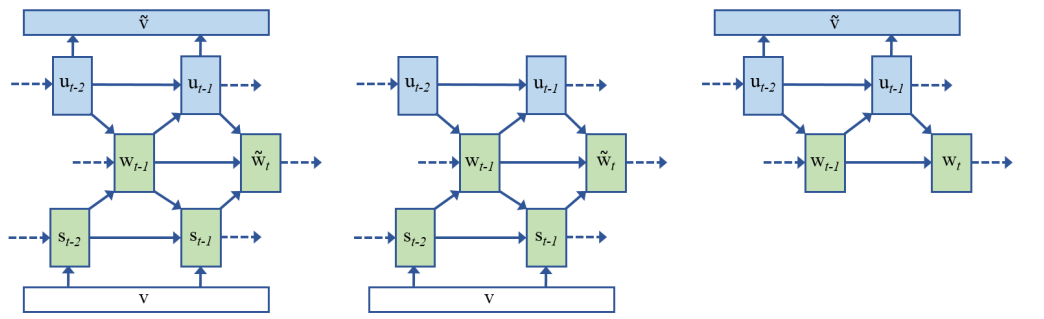
\includegraphics[scale=0.5]{Imgs/mind1.png}
\caption{ساختار کلی شبکه ارائه شده برای نگاشت دوطرفه تصاویر و جملات در پژوهش \cite{chen2015mind}}
\label{fig:4-mind1}
\end{figure}


مدل دوطرفه ارائه شده، روی مجموعه‌داده‌های \lr{MS COCO}، \lr{Flickr8k} و \lr{Flickr30K} آزمایش شده و نتایج حاصل از آن در جدول \ref{tbl:4-mind1} با نتایج روش‌های دیگر مورد مقایسه قرار گرفته‌ است.


\begin{table}[h]
\centering
\caption{نتایج عمل‌کرد مدل نگاشت دوطرفه ارائه شده در \cite{chen2015mind}}
\begin{tabular}{|c|c|c|c|c|c|c|}
\hline
نام مدل& مجموعه‌داده & \lr{‌BLEU} &مجموعه‌داده & \lr{‌BLEU} &مجموعه‌داده & \lr{‌BLEU} 
\\
\hline

\end{tabular}

\end{table}